\subsection{Driver}

The converter is not working properly in boost mode. Sometimes we managed to get some test results from it, but at some point it always stopped working. When this happened the Drv4 burned and needed to be changed. The exact reason can be due to many things and is still a concern. \ref{Voltagespike} shows the output voltage of the driver after the gate resistors R11 and R12:

\begin{figure}[H]
	\begin{center}
		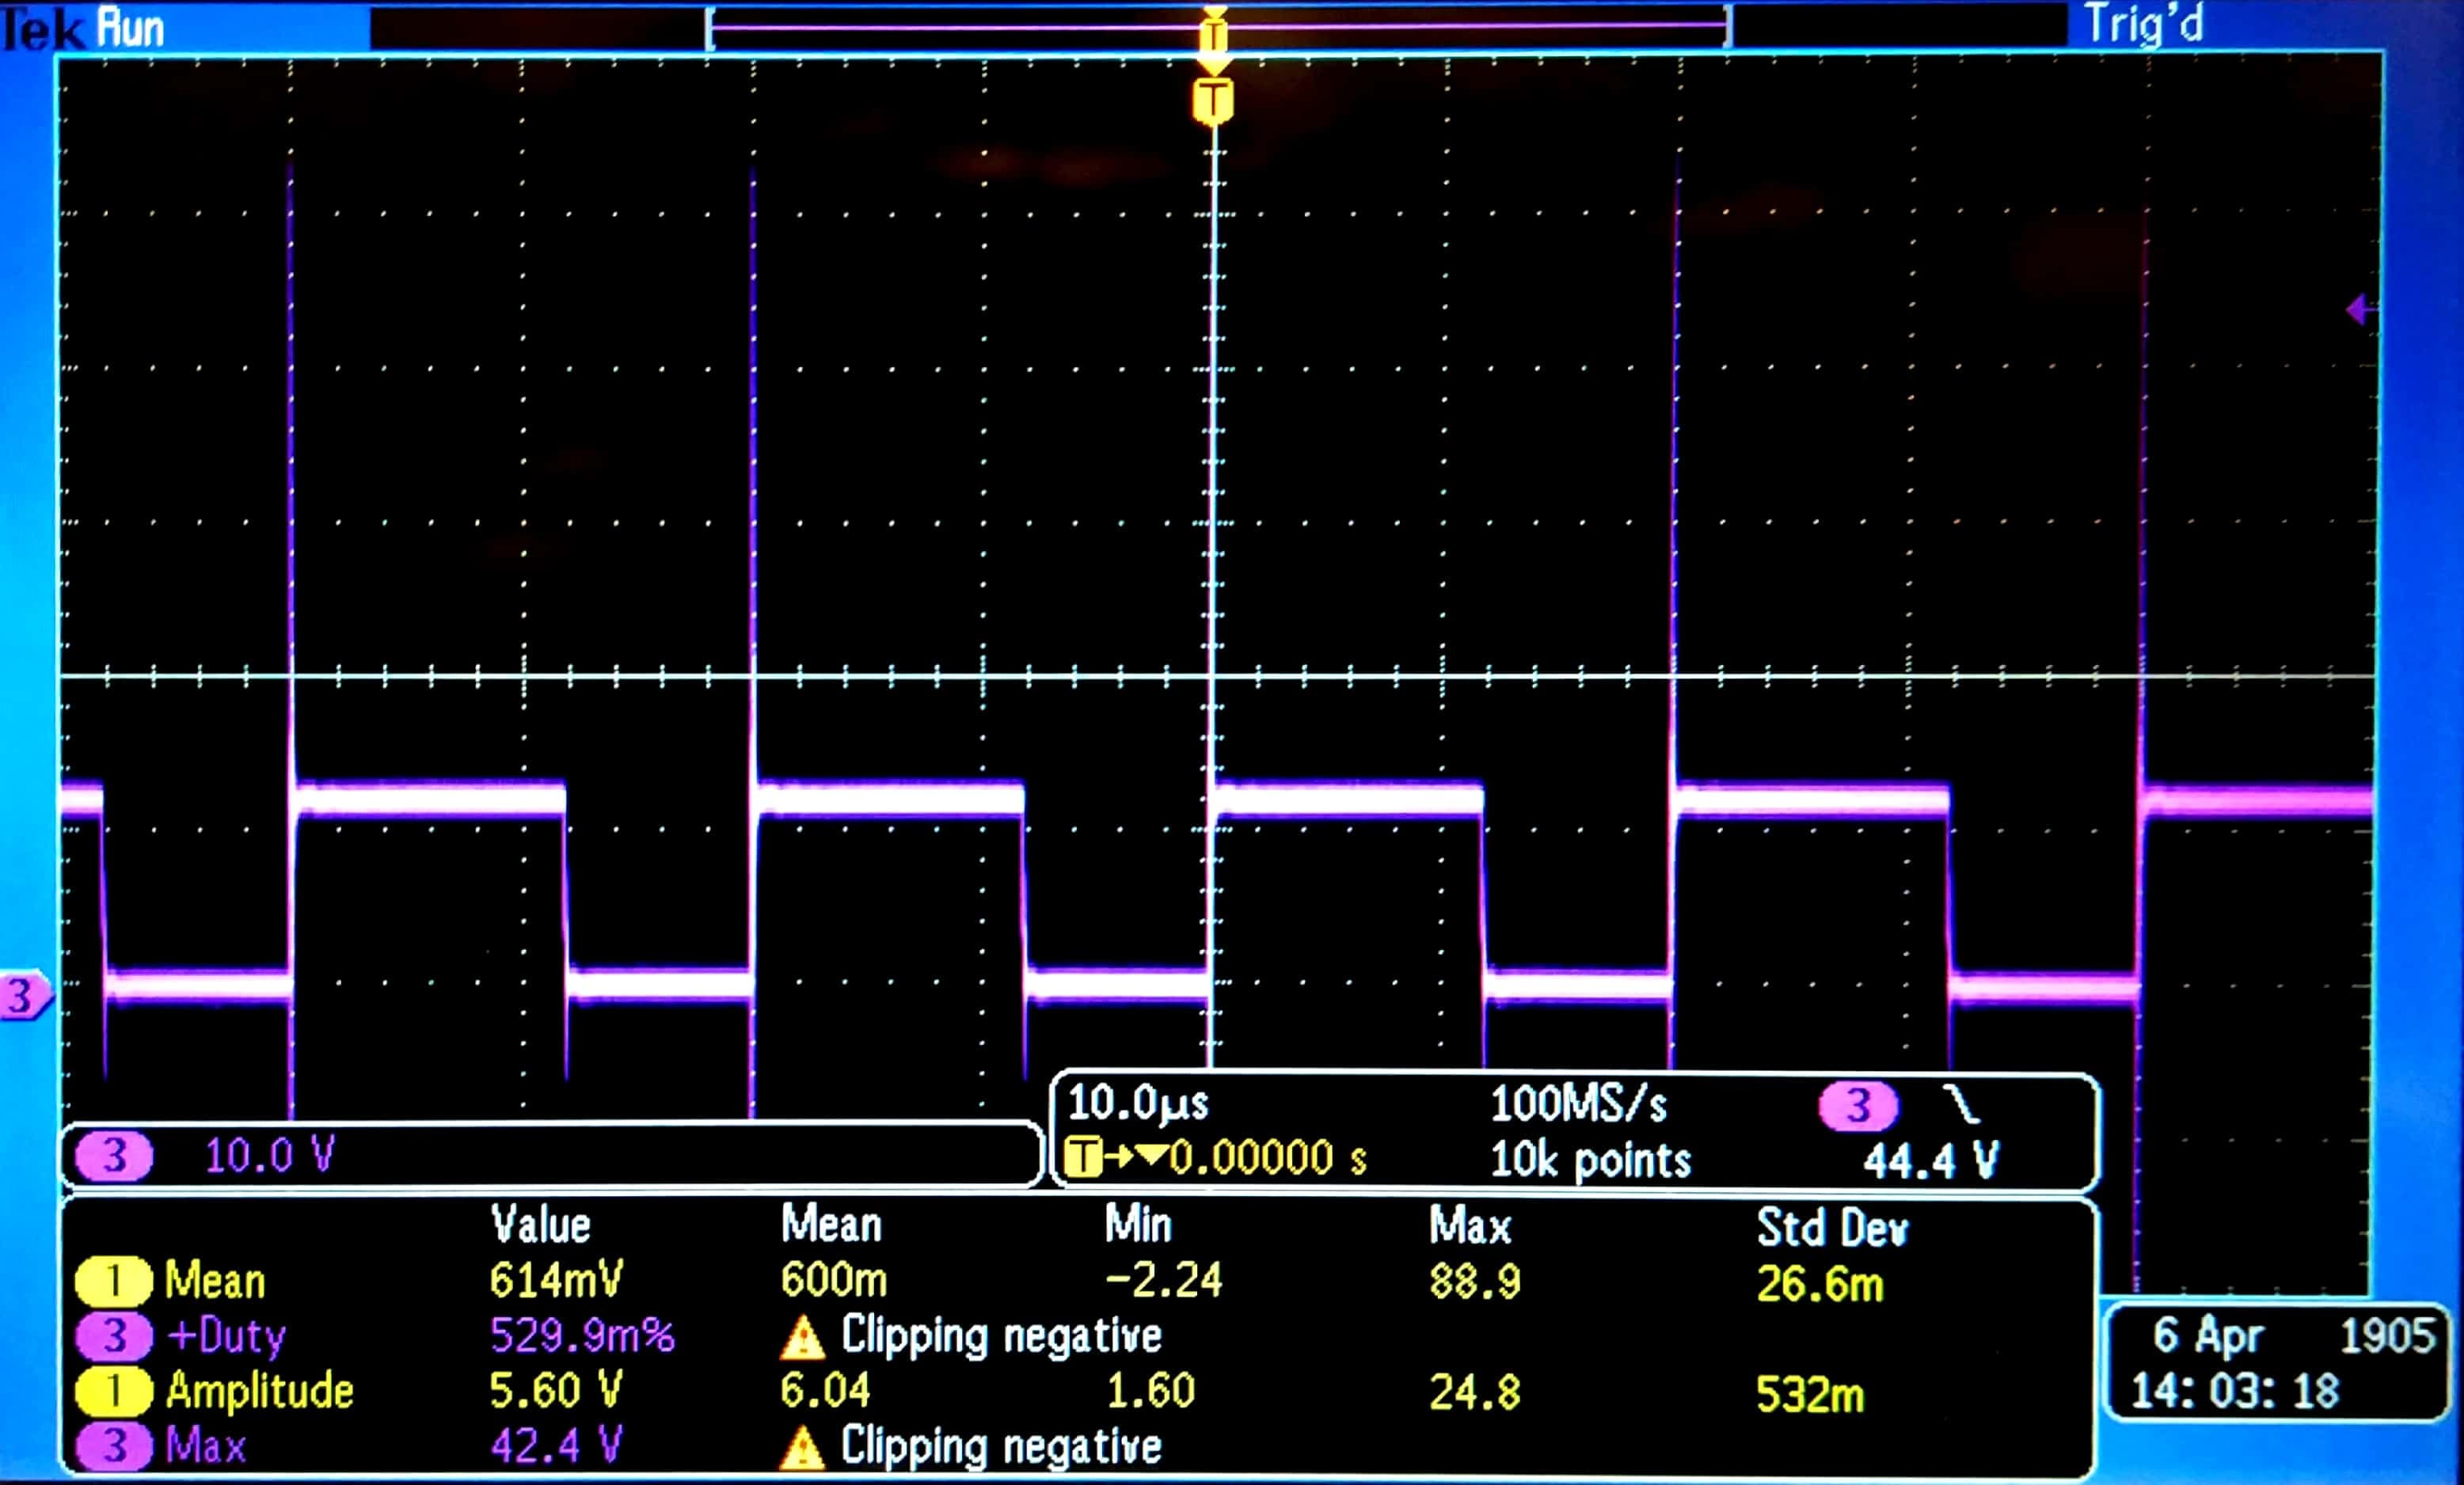
\includegraphics[width=0.7\textwidth]{../Pictures/P1/Discussion/Voltagespike.jpg}
		\caption{Output voltage of driver after gate resistors $20\Omega$}
		\label{Voltagespike}
	\end{center}	
\end{figure}    

Looking at the graph it can be seen that the switching spikes is reaching above 50V. This means that a big current will run through the driver and MOSFET while switching which might be why the driver burns. To lower these voltage spikes the gate resistors were changed to two $100\Omega$ instead. This results in the graph at \ref{Voltagespike_100}

\begin{figure}[H]
	\begin{center}
		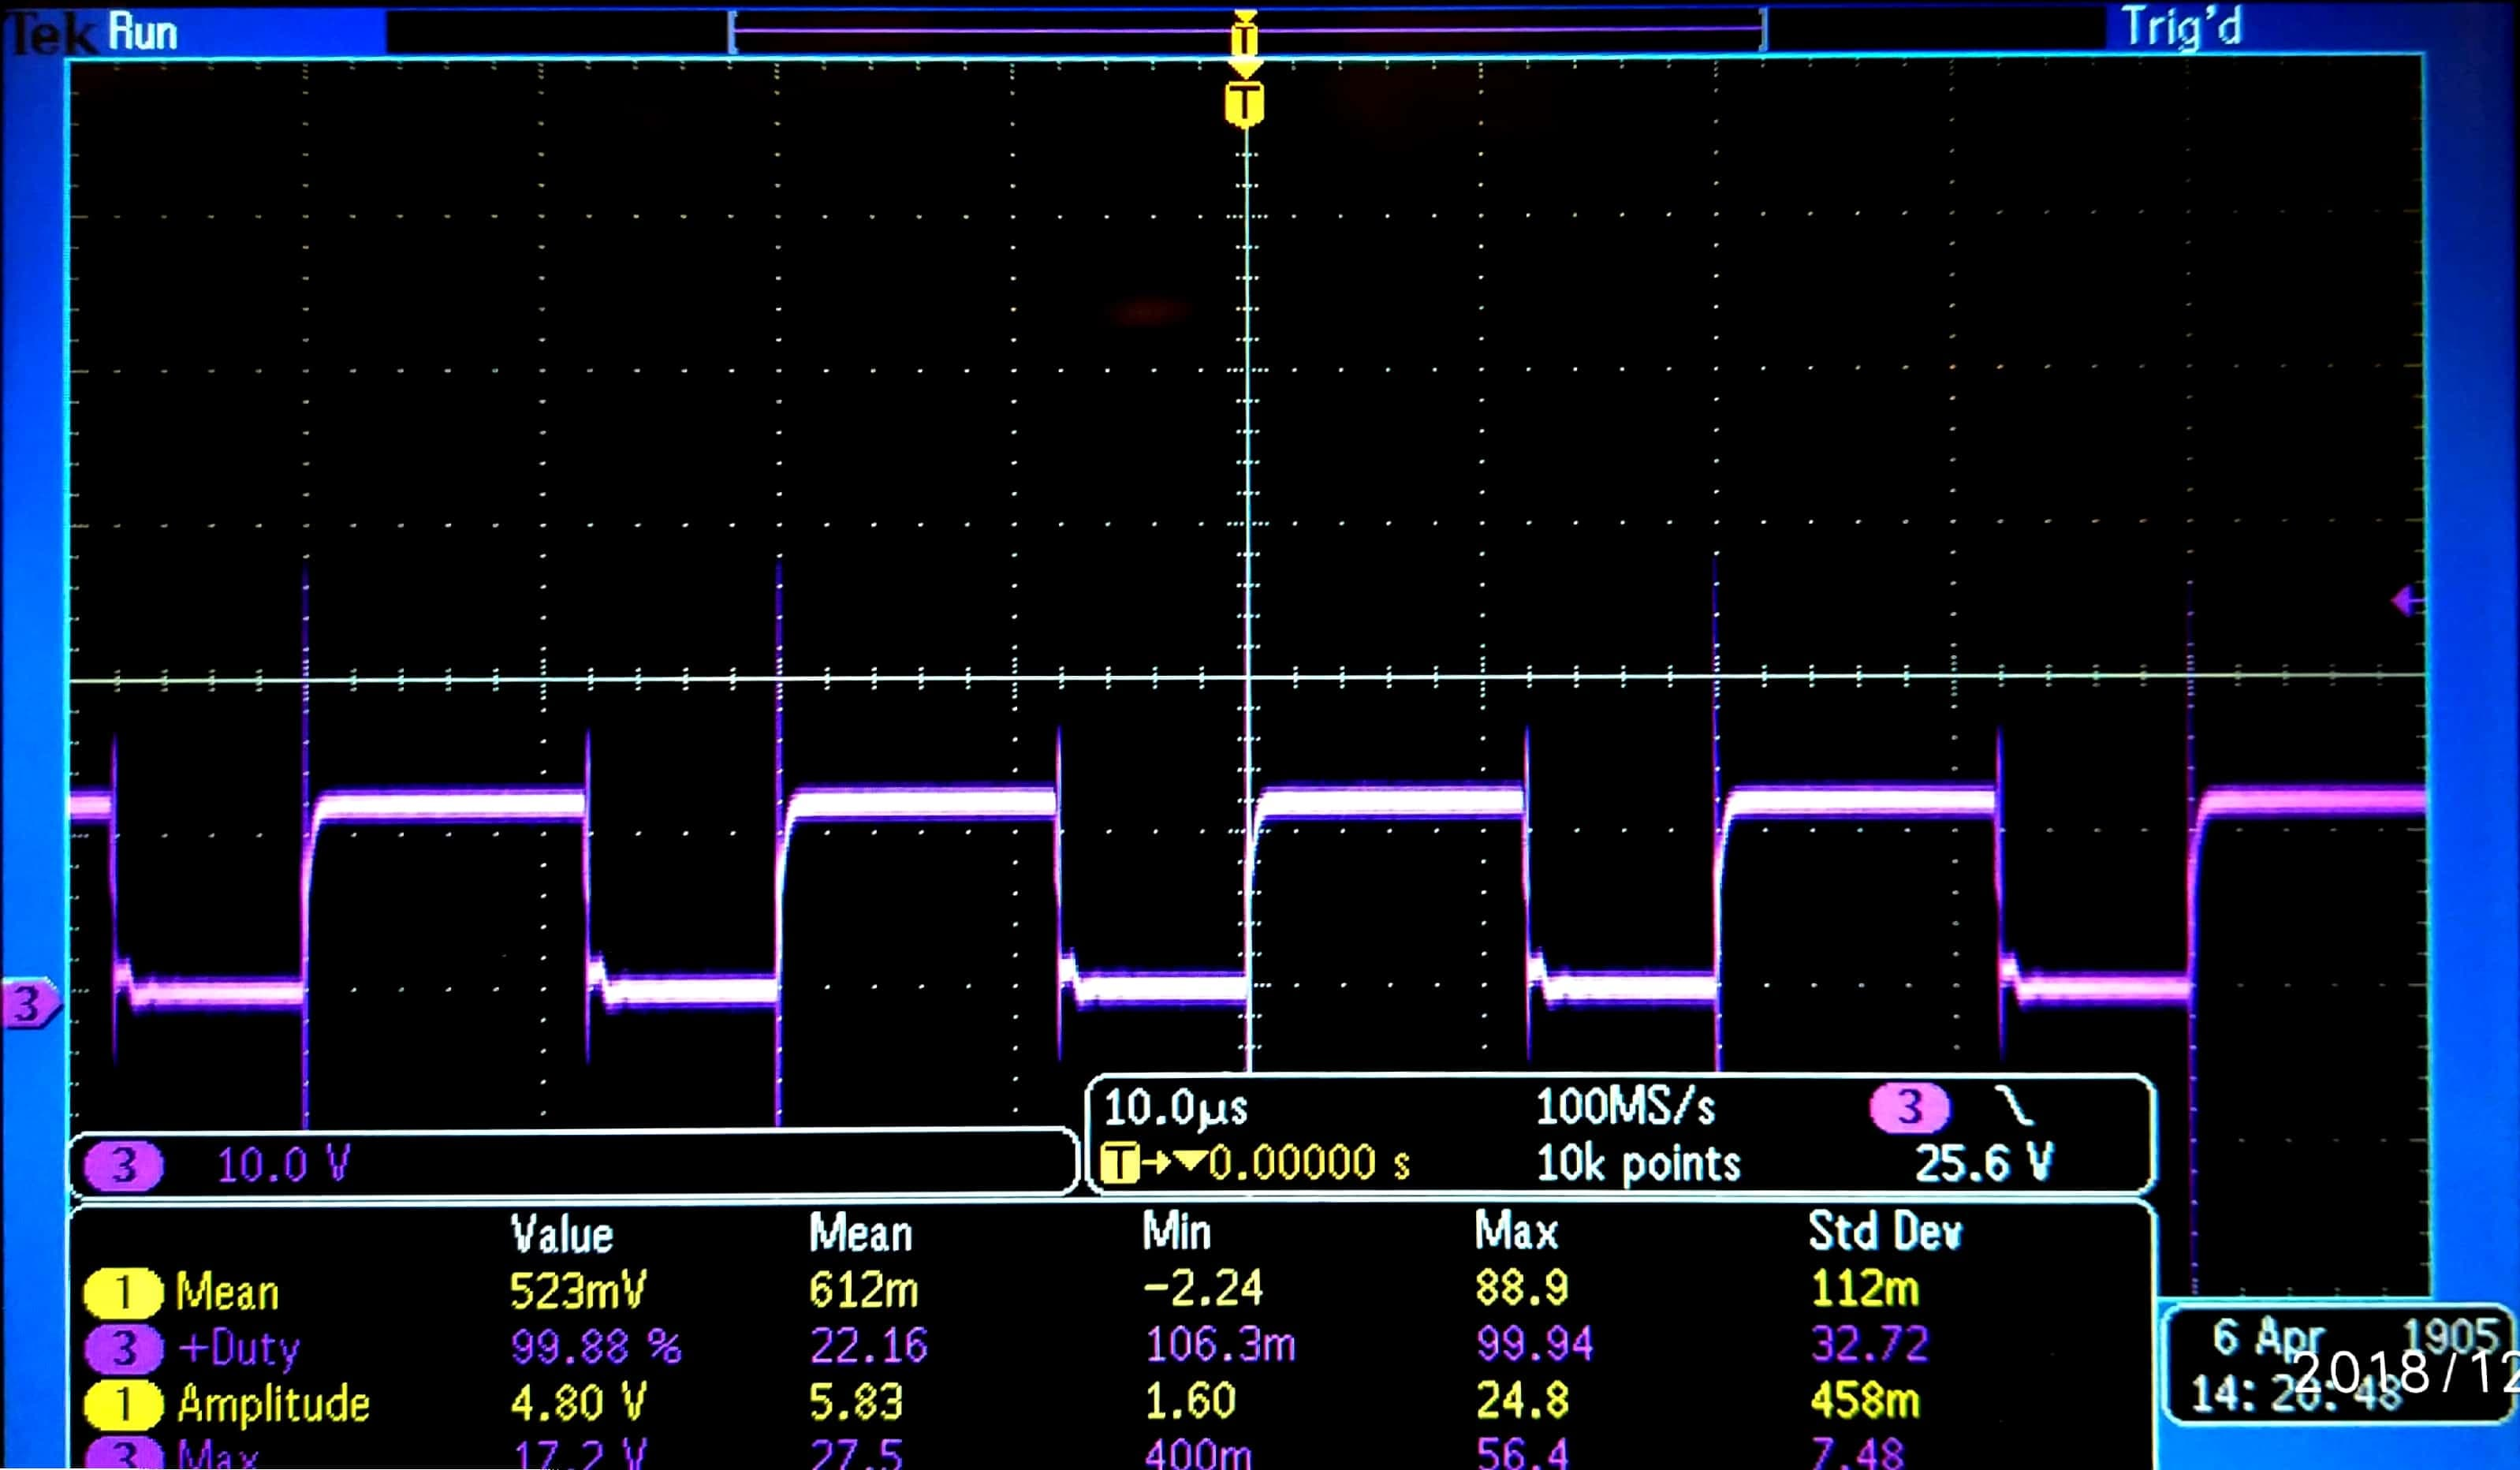
\includegraphics[width=0.7\textwidth]{../Pictures/P1/Discussion/Voltagespike_new_resistors.jpg}
		\caption{Output voltage of driver after gate resistors $100\Omega$}
		\label{Voltagespike_100}
	\end{center}	
\end{figure} 

As expected the changed resistors has decreased the voltage spikes to a bit above 20V. However, this did not solve the problem since the driver still broke. Removing the spikes completely and trying other ways to fix the problem will be done in the future.    
Because of this issue it was not possible to measure the worst case output ripple voltage of the converter which is in boost mode. Therefore the experimental result of the output voltage ripple has ben done for buck mode instead.   